\documentclass{article}
\usepackage{graphicx} % Required for inserting images
\usepackage[a4paper, total={6in, 8in}]{geometry}
\usepackage{subcaption}
\usepackage{float} % Required for positioning figures and tables at the specified location

\title{CE4046 Intelligent Agent Assignment 1}
\author{Tianrun Hu}
\date{\today}

\begin{document}

\maketitle

\section{Method of value iteration}

\subsection{Description of Implemented Solution}

\paragraph{Initialization:} The environment is pass into the function by a class contains all the walls and rewards. A SummaryWriter object from tensorboardX is created for logging purposes. A utility values array V if initialized with zeros for each state in the environment.

\paragraph{Iteration:} The update step in the value iteration algorithm is:
\[V_{k+1}(s) = max_a \sum_{s'}P(s'|s, a) [R(s, a, s'), + \gamma V_k(s')] \]

where $V_k(s)$ is the utility of state $s$ at iteration $k$, $max_a$ denotes the maximum value over all possible actions $a$, $P(s' | s, a) $ is the probability of transitioning to state $s'$ from state $s$ to state $s'$ via action $a$, $\gamma$ is the discount factor which prioritizes immediate rewards over distant rewards, $V_k(s')$ is the utility of state $s'$ at iteration $k$.

Run for 50 iterations, and keep tracking the maximum change in utility values $\delta$. If it falls below a specified threshold, indicating convergence.

\paragraph{Plotting:} Plot the values and policies calculated from the previous algorithm.

\subsection{Plot of Optimal Policy}

\begin{figure}[H]
    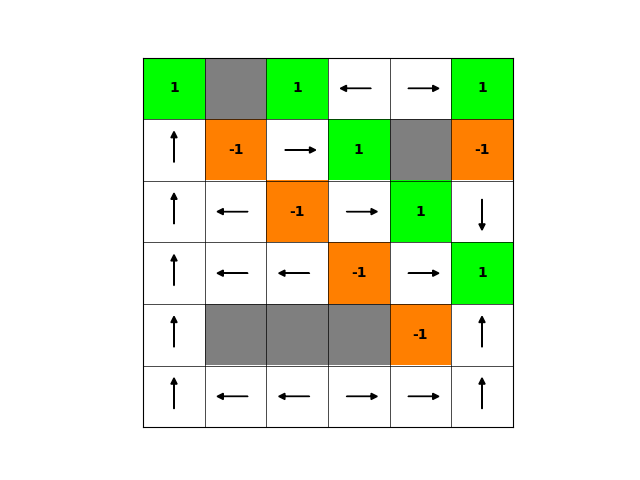
\includegraphics[width=100mm]{../asset/value_iteration_policy.png}
    \caption{Optimal policy for the gridworld environment. The arrows indicate the action to be taken in each state. The color of the arrows represent the value of the action.}
    \label{fig:value_iteration_policy}
\end{figure}

\subsection{Utility of all states}

\begin{figure}[H]
    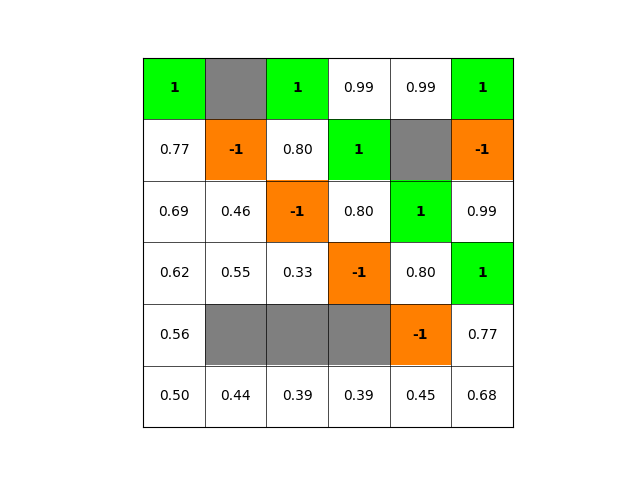
\includegraphics[width=100mm]{../asset/value_iteration_utility.png}
    \caption{Utility of all states in the gridworld environment. The color of the cells represent the value of the state.}
    \label{fig:value_iteration_utility}
\end{figure}

The more detailed value for the final utility is:

\begin{table}[H]
    \begin{tabular}{|l|l|l|l|l|l|}
        \hline
        0.0        & 0.0        & 0.0        & 0.99445061 & 0.98753071 & 0.0        \\\hline
        0.77247503 & 0.0        & 0.8        & 0.0        & 0.0        & 0.0        \\\hline
        0.68529708 & 0.4611854  & 0.0        & 0.8        & 0.0        & 0.99445061 \\\hline
        0.61840233 & 0.54986211 & 0.33239009 & 0.0        & 0.8        & 0.0        \\\hline
        0.56078941 & 0.0        & 0.0        & 0.0        & 0.0        & 0.77247503 \\\hline
        0.49686767 & 0.4406518  & 0.38504299 & 0.3947778  & 0.45040336 & 0.68411722 \\\hline
    \end{tabular}
\end{table}

\subsection{Convergence of value iteration}

\begin{figure}[H]
    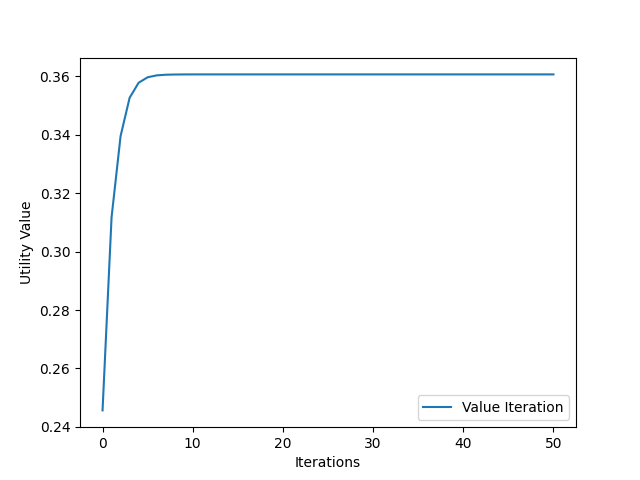
\includegraphics[width=100mm]{../asset/value_iteration_curve.png}
    \caption{Convergence of value iteration. The y-axis represents the maximum change in utility values across all states. The x-axis represents the number of iterations.}
    \label{fig:value_iteration_convergence}
\end{figure}

\section{Method of policy iteration}

\subsection{Description of Implemented Solution}

\paragraph{Initialization:} The setting is basically same with value iteration. Except here we initialize the policy as all actions are set to move right (0, 1).

\paragraph{Policy Evaluation:} For each state, the expected utility is computed based on the current policy's action, considering the probability of transitions to all possible next states and the corresponding rewards.

\paragraph{Policy iteration:} The iteration consists of two steps: evaluation and improvement.

Policy Evaluation: 
\[V^\pi (s) = \sum_{s', r} P(s', r|s, \pi(s))[r + \gamma V^\pi (s')] \]

where $V^\pi(s)$ is the utility of state $s$ under policy $\pi$, $P(s', r | s, \pi(s))$ is the probability of transitioning to state $s'$ with reward $r$ from state $s$ when following policy $\pi$. $\gamma$ is the discount factor and $\pi(s)$ is the action prescribed by policy $\pi$ in state $s$.

Policy Improvement:
\[\pi ' (s) = arg max_a \sum_{s', r} P(s', r|s, a)[r + \gamma V^\pi (s')] \]

where $pi '(s)$ is the updated action for state $s$ under the improved policy $\pi '$, $argmax_a$ denotes the action that maximizes the expected utility.

\subsection{Plot of Optimal Policy}

\begin{figure}[H]
    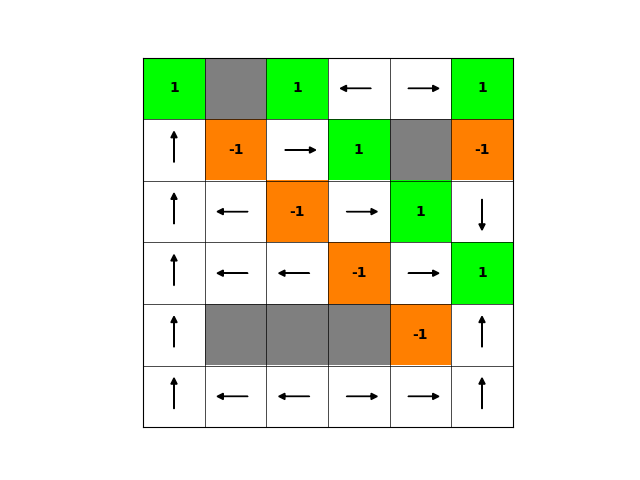
\includegraphics[width=100mm]{../asset/policy_iteration_policy.png}
    \caption{Optimal policy for the gridworld environment. The arrows indicate the action to be taken in each state. The color of the arrows represent the value of the action.}
    \label{fig:policy_iteration_policy}
\end{figure}

\subsection{Utility of all states}

\begin{figure}[H]
    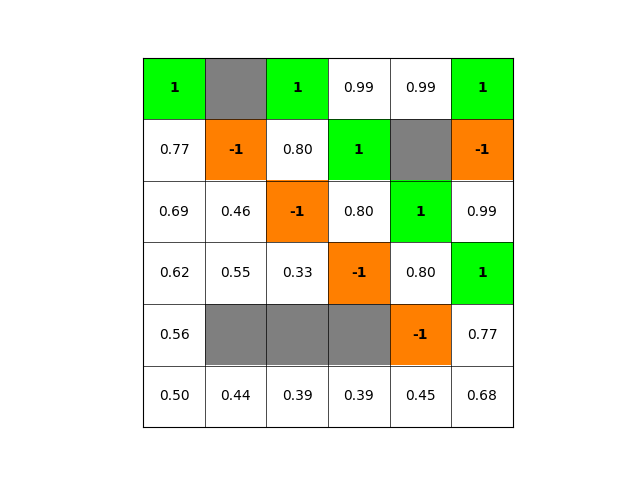
\includegraphics[width=100mm]{../asset/policy_iteration_utility.png}
    \caption{Utility of all states in the gridworld environment. The color of the cells represent the value of the state.}
    \label{fig:policy_iteration_utility}
\end{figure}

\begin{table}[H]
    \begin{tabular}{|l|l|l|l|l|l|}
        \hline
        0.0        & 0.0        & 0.0        & 0.99445061 & 0.98753071 & 0.0        \\\hline
        0.77247503 & 0.0        & 0.8        & 0.0        & 0.0        & 0.0        \\\hline
        0.68529708 & 0.4611854  & 0.0        & 0.8        & 0.0        & 0.99445061 \\\hline
        0.61840233 & 0.54986211 & 0.33239009 & 0.0        & 0.8        & 0.0        \\\hline
        0.56078941 & 0.0        & 0.0        & 0.0        & 0.0        & 0.77247503 \\\hline
        0.49686767 & 0.4406518  & 0.38504299 & 0.3947778  & 0.45040336 & 0.68411722 \\\hline
    \end{tabular}
\end{table}

It shows that in the default maze setting, the policy iteration and value iteration will converge to the same utility values.

\subsection{Convergence of policy iteration}

\begin{figure}[H]
    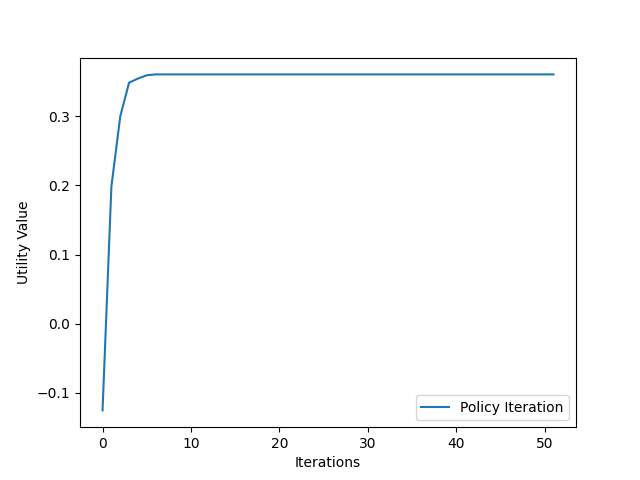
\includegraphics[width=100mm]{../asset/policy_iteration_curve.png}
    \caption{Convergence of policy iteration. The y-axis represents the maximum change in utility values across all states. The x-axis represents the number of iterations.}
    \label{fig:policy_iteration_convergence}
\end{figure}

\section{Bonus questions}

\subsection{Environment generation}

\paragraph{Randomly generated environment:} The environment is generated by randomly placing walls and rewards in the gridworld. The number of walls and rewards are specified by the user. The rewards are placed randomly in the environment, and the walls are placed randomly in the environment. The generated environment is save as yaml file in config folder. Here are some examples of the generated environment:

\begin{figure}[H]
    \centering
    \begin{subfigure}{.5\textwidth}
        \centering
        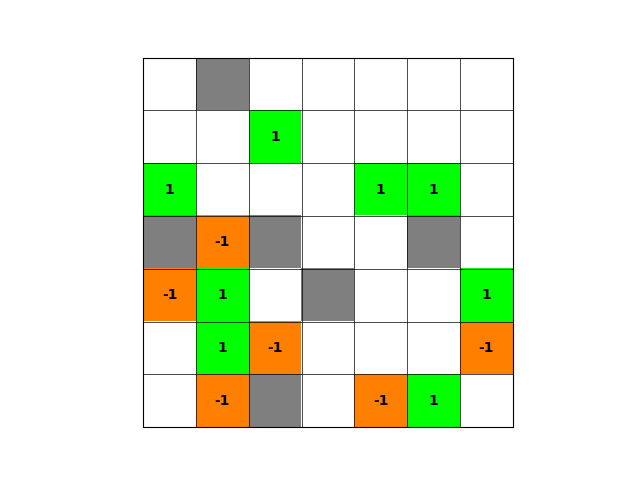
\includegraphics[width=60mm]{../results/maze_size_7/env.png}
        \caption{Maze size 7}
        \label{fig:random_env_1}
    \end{subfigure}%
    \begin{subfigure}{.5\textwidth}
        \centering
        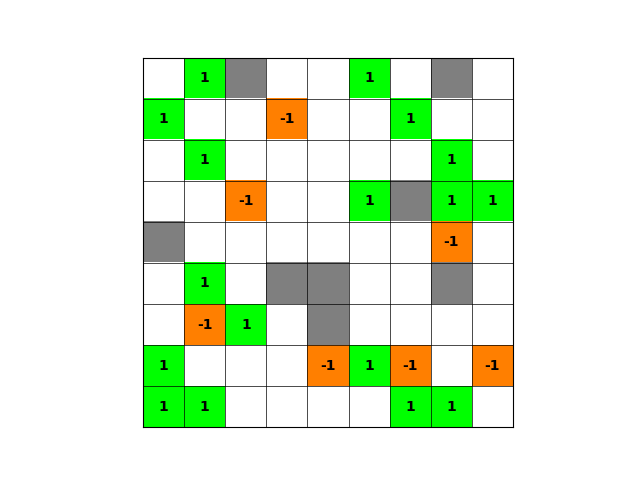
\includegraphics[width=60mm]{../results/maze_size_9/env.png}
        \caption{Maze size 9}
        \label{fig:random_env_2}
    \end{subfigure}
\end{figure}
\begin{figure}[H]
    \begin{subfigure}{.5\textwidth}
        \centering
        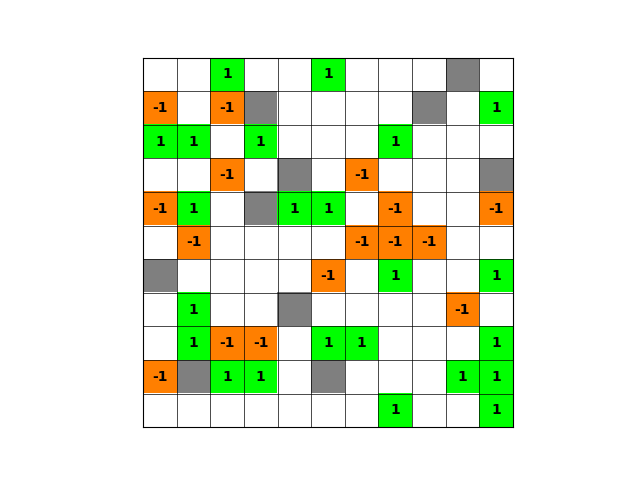
\includegraphics[width=60mm]{../results/maze_size_11/env.png}
        \caption{Maze size 11}
        \label{fig:random_env_3}
    \end{subfigure}
    \begin{subfigure}{.5\textwidth}
        \centering
        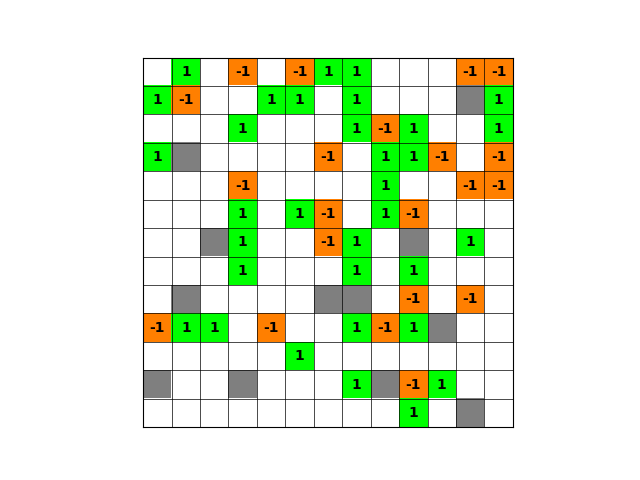
\includegraphics[width=60mm]{../results/maze_size_13/env.png}
        \caption{Maze size 13}
        \label{fig:random_env_4}
    \end{subfigure}
\end{figure}
\begin{figure}[H]
    \begin{subfigure}{.5\textwidth}
        \centering
        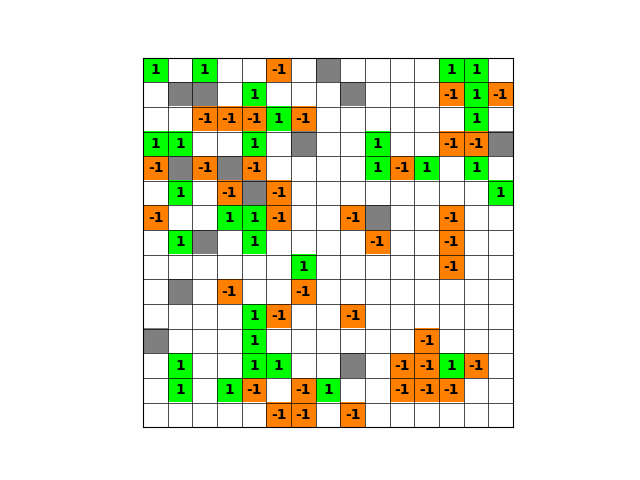
\includegraphics[width=60mm]{../results/maze_size_15/env.png}
        \caption{Maze size 15}
        \label{fig:random_env_5}
    \end{subfigure}
    \begin{subfigure}{.5\textwidth}
        \centering
        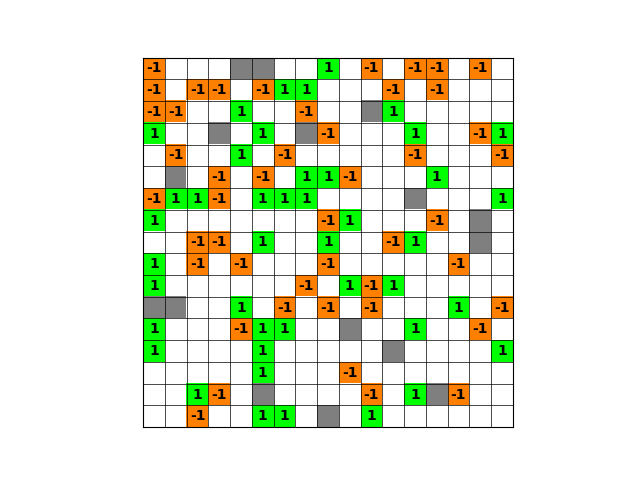
\includegraphics[width=60mm]{../results/maze_size_17/env.png}
        \caption{Maze size 17}
        \label{fig:random_env_6}
    \end{subfigure}
    \caption{Randomly generated environments.}
\end{figure}

\subsection{Comparison of value iteration and policy iteration}

\paragraph{Convergence among different maze complexity:} The convergence of value iteration and policy iteration for different maze size is shown in Figure \ref{fig:value_iteration_convergence} and Figure \ref{fig:policy_iteration_convergence}.

\begin{figure}[H]
    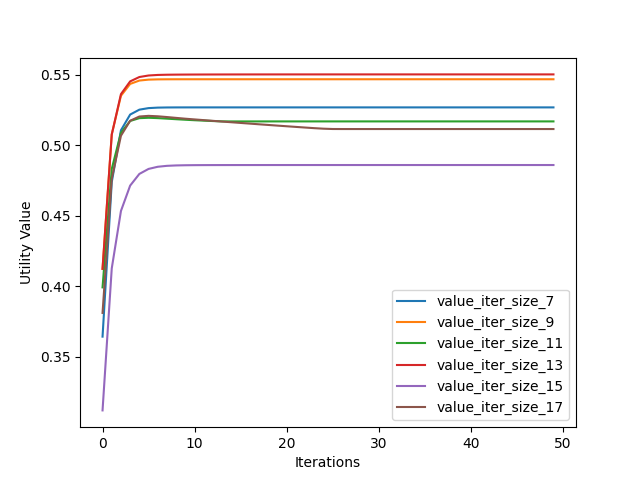
\includegraphics[width=100mm]{../results/value_iteration_curves.png}
    \caption{The value iteration curves for different maze size.}
    \label{fig:value_iteration_convergence}
\end{figure}

\begin{figure}[H]
    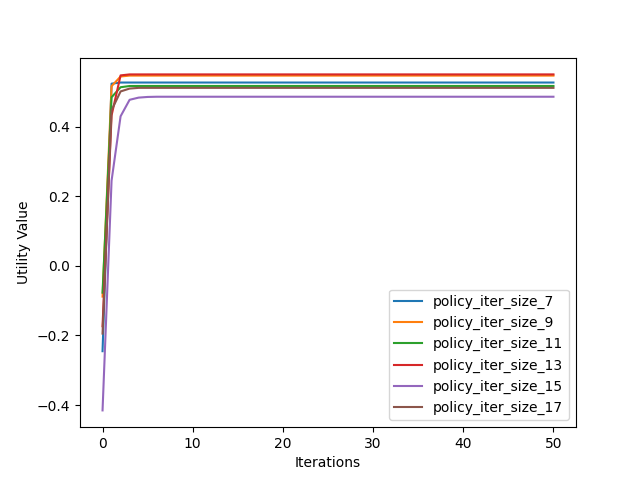
\includegraphics[width=100mm]{../results/policy_iteration_curves.png}
    \caption{The policy iteration curves for different maze size.}
    \label{fig:policy_iteration_convergence}
\end{figure}

It shows that the maze complexity will affect the convergence of value iteration and policy iteration. The larger the maze size, the slower the convergence, and the lower final utility values will be.

\end{document}
